\section{Theorie}
\label{sec:Theorie}

\cite{sample}

\subsection{Zielsetzung}
\label{subsec:Zielsetzung}

Ziel des Versuches ist, die Funktionsweise der einzelnen Komponenten des Lock-In-Verstärkers
zu verstehen.\\


\subsection{Funktionsweise}
\label{subsec:Funktionsweise}

Der Lock-In-Verstärker wird verwendet, um verrauschte Signale zu messen. \\
Er enthält einen sogenannten phasenempfindlichen Detektor, einen Bandpassfilter, Mischer, 
Phasenschieber und einen CR-Tiefpassfilter.\\
Dabei muss eine Referenzfrequenz $\omega_0$ gewählt werden, mit der das Signal moduliert wird.\\


Ein eingehendes Signal durchläuft zuerst den Bandpassfilter, welcher zu hohe und zu niedrige 
Frequenzen nicht passieren lässt. So wird das Rauschen um die Referenzfrequenz herum
entfernt. \\
Dann multipliziert der Mischer das Signal mit einem Referenzsignal 
$U_{ref}$ gleicher Frequenz ($\omega_0$).\\
Daraufhin werden mit Hilfe des Phasenschiebers die Signale synchronisiert.\\
Über die integrierende Funktion des RC-Tiefpasses können Rauschbeträge herausgemittelt werden.
Die Zeitkostante $\tau = RC$ moduliert hier die Bandbreite des Rauschens. \\
Das Ausgangssignal einer eingehenden Sinusspannung ergibt sich beispielsweise
dann zu 

\begin{equation*}
    U_{out} \propto U_0 cos( \Phi).
\end{equation*}


\begin{figure}[H]
    \centering
    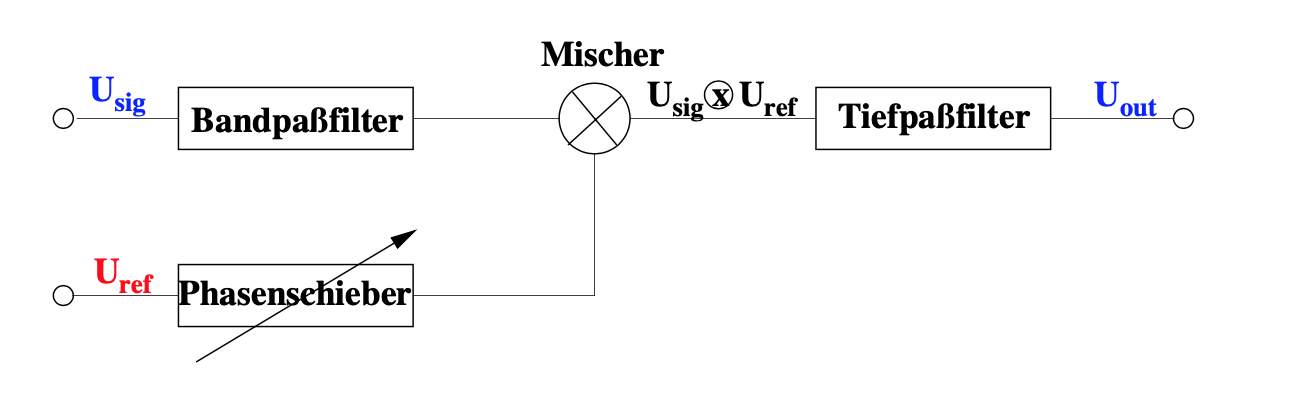
\includegraphics[scale=1]{content/lock_in_prinzip.png}
    \caption{Der schematische Aufbau des Lock-In-Verstärkers. Quelle:\cite{sample}}
    \label{fig:Prinzip_lock_in}
\end{figure}

